Las mediciones de los siete caminos están en la tabla \ref{tab:datos}. La columna de ajuste indica qué tan lejos queda cada punto de P4, el que dio el camino más corto, y se calculó como $x - 12.2$ cm.

\begin{center}
\begin{tabular}{cccc}
\hline
Punto & $x$ (cm) & $L$ (cm) & Ajuste (cm) \\
\hline
P1 & 17.3 & 40.4 & 5.1 \\
P2 & 16.1 & 39.7 & 3.9 \\
P3 & 14.6 & 39.5 & 2.4 \\
P4 & 12.2 & 39.4 & 0.0 \\
P5 & 7.2  & 40.5 & $-5.0$ \\
P6 & 4.5  & 42.1 & $-7.7$ \\
P7 & 0.0  & 45.6 & $-12.2$ \\
\hline
\end{tabular}
\captionof{table}{Distancia $x$ de cada punto al origen, longitud total $L$ del camino A', P, B y posición de cada punto respecto a P4.}
\label{tab:datos}
\end{center}

A simple vista ya se nota que la longitud baja, toca fondo y vuelve a subir. Para verlo mejor hicimos la gráfica de la figura \ref{fig:grafica}, a la que agregamos una parábola de ajuste por mínimos cuadrados:
\begin{equation}
L(x) = 0.0393\,x^2 - 0.9927\,x + 45.651 ,
\label{eq:ajuste}
\end{equation}
con un coeficiente de determinación $R^2 = 0.9976$.

\begin{center}
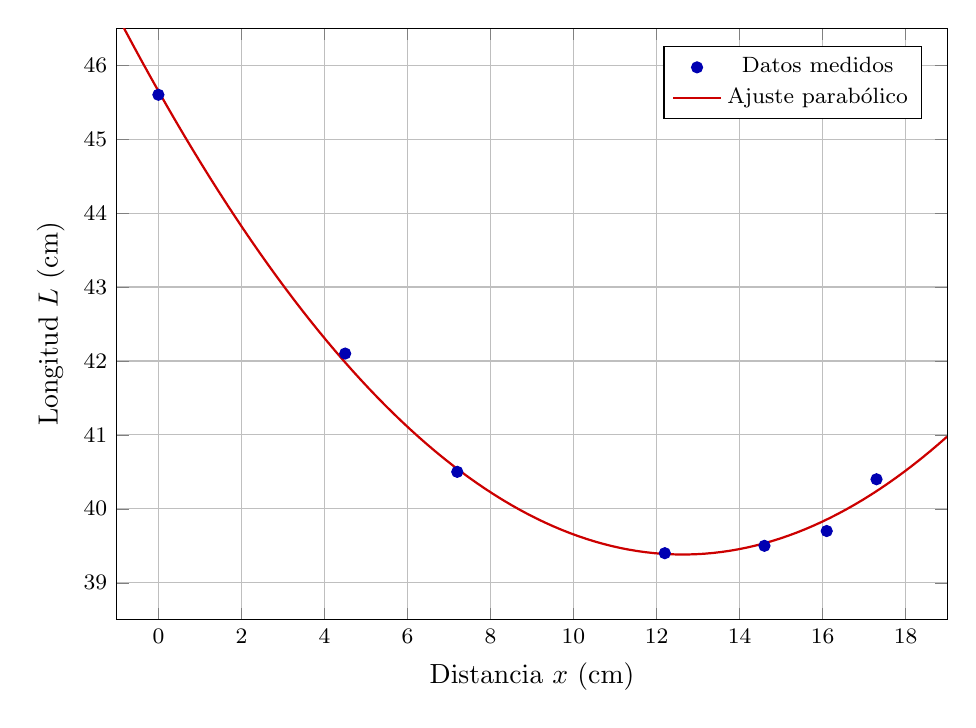
\begin{tikzpicture}
\begin{axis}[
    width=\columnwidth,
    height=0.75\columnwidth,
    xlabel={Distancia $x$ (cm)},
    ylabel={Longitud $L$ (cm)},
    xmin=-1, xmax=19,
    ymin=38.5, ymax=46.5,
    grid=major,
    legend pos=north east,
    legend style={font=\footnotesize},
    tick label style={font=\footnotesize},
]
\addplot[only marks, mark=*, color=blue!70!black] coordinates {
    (17.3,40.4) (16.1,39.7) (14.6,39.5) (12.2,39.4)
    (7.2,40.5) (4.5,42.1) (0,45.6)
};
\addlegendentry{Datos medidos}
\addplot[domain=-1:19, samples=100, thick, color=red!80!black]
    {0.0393*x^2 - 0.9927*x + 45.651};
\addlegendentry{Ajuste parabólico}
\end{axis}
\end{tikzpicture}
\captionof{figure}{Longitud del camino contra la distancia $x$ del punto de contacto al origen. Los puntos son los datos medidos y la curva roja es la parábola de la ecuación \eqref{eq:ajuste}.}
\label{fig:grafica}
\end{center}

Derivando la ecuación \eqref{eq:ajuste} e igualando a cero se obtiene la posición del mínimo:
\begin{equation}
\frac{dL}{dx} = 0.0786\,x - 0.9927 = 0 ,
\label{eq:minimo}
\end{equation}
y al despejar queda $x_{min} = 12.63$ cm.
Sustituyendo ese valor en la parábola, la longitud mínima resulta $L_{min} = 39.38$ cm.

Medido directamente, el mínimo fue de 39.4 cm en P4, que está en $x = 12.2$ cm. Ahí la línea que va de A' a P4 y la que va de P4 a B quedaron prácticamente como una sola recta, y fue en ese punto donde el ángulo de llegada y el de salida se vieron iguales en el papel.
